

%% josis.tex 1.4   2016-09-15    JoSIS latex template
%------------------------------------------------------------------
% Filename: josis_template.tex
%
% This file is intended as a template for typesetting articles for the
%
%                        Journal of Spatial Information Science.
%
% Please edit this template to generate your own formatted manuscripts
% for submission to JOSIS. See http://josis.org for further details.
%


%%% JOSIS checks in typesetting
%%% * All titles and sections lower case *EXCEPT short title  [ ]
%%% * Remove author postal addresses, only have geographic places and institutions [ ] 
%%% * Consistent use of Section, Figure, Table (capitalized and in full) [ ]
%%% * 10 keywords (and all lower case) [ ]
%%% * Remove all avoidable footnotes [ ]
%%% * Use double quotation marks (``'' not "" or `') [ ]
%%% * Punctuation inside quotations [ ]
%%% * E.g. and i.e. followed by comma [ ]
%%% * cf. followed by tilde [ ]
%%% * Itemize and enumerate correctly punctuated [e.g., "1. x, 2. y, and 3. x." ]
%%% * And/or lists using American English punctuation (e.g., "x, y, and z") [ ] 
%%% * Bibliography (e.g., en-dashes for number ranges, consistent "Proc.~" for Proceedings of..., etc.) []
%%% * Acknowledgment style use section* [ ] 
%%% * et al. no italics, but with dot  [ ] 
%%% * All captions end with full stop  [ ] 
%%% * Table captions under, not over table  [ ]
%%% * Adjust urls with burlalt [ ] 
%%% * Check correct use of hyphens, emdashes, endashes  [ ]
%%% * Perform spell check  [ ] 

%%% JOSIS checks directly before publication 
%%% Check DOI, page numbers on article and web site. [ ]
%%% Update web site with final title, abstract, keywords. [ ] 
%%% Build with distiller for DOI links. [ ]


% Required documentclass definition for JOSIS
\documentclass{josis}
\usepackage{hyperref}
\usepackage[hyphenbreaks]{breakurl}
\usepackage{booktabs}
\usepackage{stmaryrd}
\usepackage[T1]{fontenc}
\usepackage{cite}
\usepackage{subcaption}

% Suggested packages for algorithm formatting
\usepackage{algorithm}
%\usepackage{algorithmic}
\usepackage{algpseudocode}
\usepackage{pythonhighlight}

\usepackage{amssymb,amsmath}
%\usepackage[table]{xcolor}
\usepackage{lastpage}
\renewcommand{\topfraction}{0.9} 
\renewcommand{\textfraction}{0.1}
% Page setup and overhangs
\sloppy
\widowpenalty=10000
\clubpenalty=10000
\hyphenpenalty=75

% Article details for accepted manuscripts will be added by editorial staff
% Omit year if article in press
% Omit number if article under review
\josisdetails{%
   number=2, year=2024, firstpage=1, lastpage=\pageref{LastPage}, 
  doi={IUCP-2024},
  % received={December 24, 2015}, 
   %returned={February 25, 2016},
   %revised={July 13, 2016},
   %accepted={September 5, 2016},
   }

%\newcommand{\mydoi}[1]{\href{http://dx.doi.org/#1}{doi:\protect\detokenize{#1}}}

%\renewcommand{\UrlLeft}{http:\sslash}
%\DeclareUrlCommand\myurl{\def\UrlLeft{}\def\UrlRight{}%
%\urlstyle{tt}}

\urlstyle{rm}
\makeatletter
% Inspired by http://anti.teamidiot.de/nei/2009/09/latex_url_slash_spacingkerning/
% but slightly less kern and shorter underscore
\let\UrlSpecialsOld\UrlSpecials
\def\UrlSpecials{\UrlSpecialsOld\do\/{\Url@slash}\do\_{\Url@underscore}}%
\def\Url@slash{\@ifnextchar/{\kern-.11em\mathchar47\kern-.2em}%
    {\kern-.0em\mathchar47\kern-.08em\penalty\UrlBigBreakPenalty}}
\def\Url@underscore{\nfss@text{\leavevmode \kern.06em\vbox{\hrule\@width.3em}}}
\makeatother

\hypersetup{
colorlinks=true,
linkcolor=black,
citecolor=black,
urlcolor=black
} 

% Add the running author and running title information
\runningauthor{\begin{minipage}{.9\textwidth}\centering Er. Veena A Kumar,Aiswarya Arun, Abna EV , Bhagya Suresh Kumar \end{minipage}}
\runningtitle{Customer Segmentation}

% Document begins
\begin{document}
%\setcounter{page}{33}


% Insert your own title
\title{Customer Segmentation Using Clustering}

% Insert your manuscipts authors, affiliations, and addresses
\author{Er. Veena A Kumar}
\author{Aiswarya Arun}
\author{Abna EV}
\author{Bhagya Suresh Kumar}\affil{Saintgits Group of Institutions, Kottayam, Kerala}
\date{}
\maketitle
\section{Abstract}
This project focuses on customer segmentation for targeted marketing, utilizing demographic and purchasing data. It employs K-means clustering, comparing with hierarchical clustering,GMM,Agglomerative clustering and DBSCAN. Preprocessing tackles missing values and duplicates, identifying segments based on income, spending, and responsiveness to promotions. The goal is to refine marketing strategies and products. Despite limitations, like K-means sensitivity to initial conditions, the project highlights the value of advanced clustering for informed decision-making and enhanced customer satisfaction.

\section{Keywords}Customer Segmentation, Targeted Marketing Strategies, Demographic Information, Purchasing Behavior, K-means Clustering, Income Analysis, Spending Behavior, Promotional Campaigns,Marketing Optimization, Advanced Clustering Techniques, Customer Satisfaction
% Your main text begins here. 
\section{Introduction}
In today's dynamic business landscape, understanding customer behavior stands as a pivotal challenge. This report delves into the intricate realm of customer segmentation, a cornerstone strategy in contemporary marketing. By leveraging advanced clustering algorithms such as K-means, hierarchical clustering, and others, this study aims to uncover actionable insights from a comprehensive dataset comprising demographic details and purchasing behaviors.

The primary objective is to refine marketing strategies by identifying distinct customer segments characterized by unique preferences and behaviors. Through meticulous data preprocessing techniques, including duplicate elimination and missing value imputation, the integrity of the analyses is ensured, laying the foundation for robust clustering outcomes.

As the complexities of various clustering methodologies are navigated, challenges and limitations inherent in each approach are encountered. Nonetheless, the endeavor is driven by a commitment to uncover the transformative potential of advanced data clustering in understanding customer behavior.

Ultimately, the findings from this study hold the promise of empowering businesses to tailor their marketing efforts with precision, leading to enhanced customer engagement and satisfaction. This report serves as a testament to the intersection of data science and marketing, offering valuable insights that can inform strategic decision-making in today's competitive market landscape.
\section{Literature Review}
Customer segmentation is vital, especially in times of crisis like the pandemic, where it can mean the difference between business survival and closure. Businesses that effectively segmented their customer base thrived while others struggled. Segmentation allows targeting specific audiences, optimizing marketing efforts, and tailoring services. Traditional segmentation methods face challenges with large datasets, but advancements in big data and machine learning offer solutions like k-means clustering. This technique efficiently groups similar customers, enabling personalized marketing and service strategies. Jiang and Tuzhilin (2009) proposed K-Classifiers to optimize segmentation further, focusing resources on high-profit customers. Other studies, such as He and Li (2016) and Cho and Moon (2013), highlight the importance of segmentation in understanding customer needs and behavior.In essence, customer segmentation is not just a strategy; it's a lifeline for businesses seeking stability and growth in uncertain times.


\section{Methodology}

The customer segmentation project begins with data collection and preprocessing. Clustering algorithms like K-means, Hierarchical, DBSCAN, GMM, and Agglomerative Clustering are utilized to segment customers based on demographic and behavioral data. After evaluating cluster coherence, targeted marketing strategies are developed for each segment, integrated into initiatives, and findings are reported to stakeholders for adaptive marketing efforts.
\subsection{Dataset}With 2240 rows and 29 columns, the dataset contains customer attributes and behaviors. Descriptive statistics reveal insights into birth years, income, household composition, purchase recency, spending patterns, and campaign response indicators. These statistics offer a concise glimpse into the dataset's composition and feature distribution, crucial for analysis and modeling.

\subsection{K-means Clustering Algorithm}

K-means Clustering is a clustering algorithm in which data points, along with their dataset and features, are categorized into clusters based on their similarities. The algorithm forms K clusters based on similarity, utilizing the Euclidean distance measurement method.

\begin{itemize}
    \item \textbf{Step 1: Initialization}
    
    In the first step, k points are randomly initialized. This step is crucial as the selection of initial centroids can impact the convergence and final clustering results. Various initialization techniques, such as random initialization or k-means++ initialization, aim to improve the quality of the initial centroids.
    
    \item \textbf{Step 2: Assignment}
    
    The K-means classifier categorizes each data point to its nearest mean and rewrites the mean's coordinates. This step involves calculating the distance between each data point and the centroids and assigning the data point to the cluster with the nearest centroid. After assigning all data points to clusters, the centroids are updated to reflect the mean position of the data points within each cluster.
    
    \item \textbf{Step 3: Iteration}
    
    Iteration continues until all data points are classified. In each iteration, data points may be reassigned to different clusters as centroids are updated, aiming to minimize the within-cluster sum of squares, which measures the compactness of clusters. Common stopping criteria include a maximum number of iterations or convergence of centroids.
    
    \item \textbf{Step 4: Data Visualization}
    
    Once the clusters have been formed, data visualization techniques can be employed to understand and interpret the clustering results. Visualization methods such as scatter plots, heatmaps, or silhouette plots can help visualize the distribution of data points within clusters and assess the separation between clusters. By visualizing the clusters, the marketing team can gain insights into the characteristics and behavior of different customer segments. This understanding can inform targeted marketing strategies tailored to each cluster's preferences and needs, ultimately leading to more effective customer engagement and satisfaction.
\end{itemize}



\section{Implementation}

\begin{figure}
    \centering
    \begin{subfigure}[b]{0.45\textwidth}
        \centering
        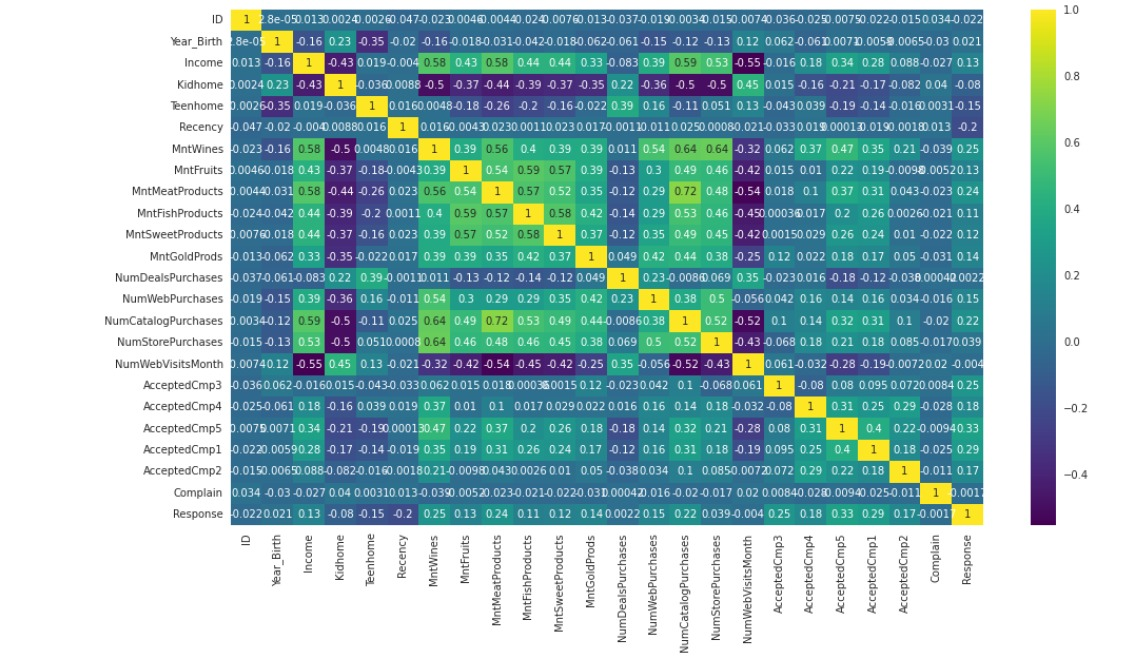
\includegraphics[width=\textwidth]{heatmap.jpeg}
        \caption{Heatmap}
        \label{fig:subfig3}
    \end{subfigure}
    \hfill
    \begin{subfigure}[b]{0.45\textwidth}
        \centering
        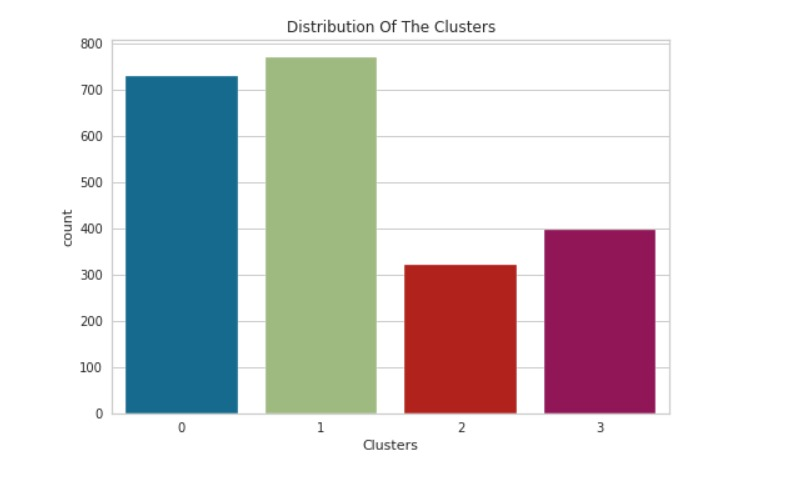
\includegraphics[width=\textwidth]{distribution.jpeg}
        \caption{Distribution of clusters}
        \label{fig:subfig3}
    \end{subfigure}
    \hfill
    \begin{subfigure}[b]{0.45\textwidth}
        \centering
        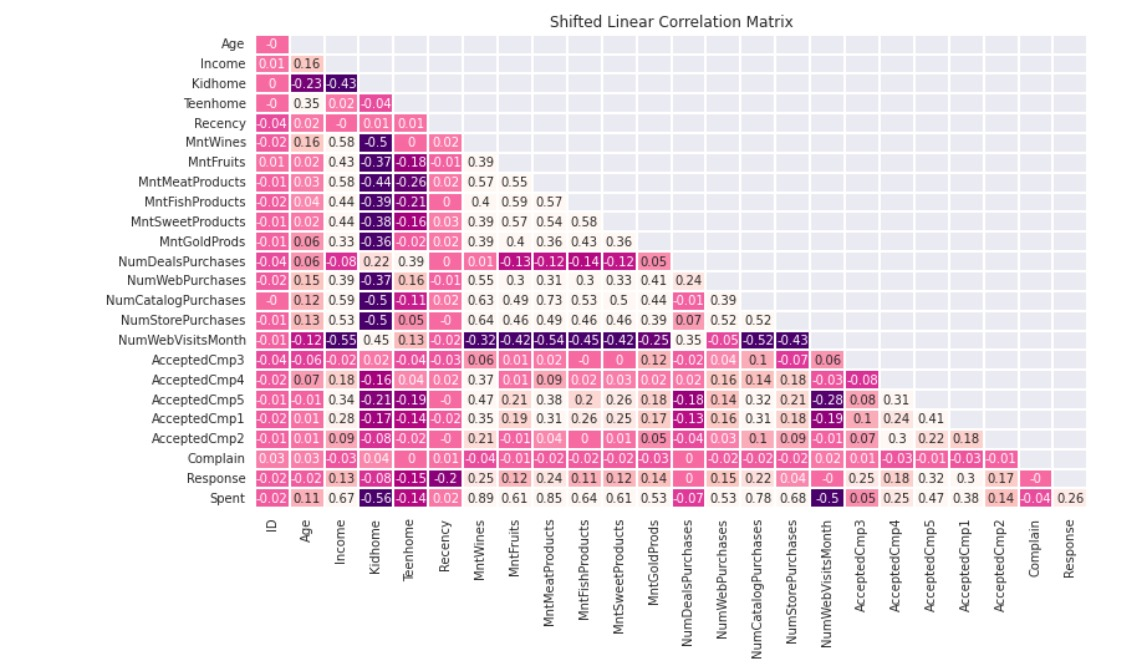
\includegraphics[width=\textwidth]{correlation_Matrix.jpeg}
        \caption{Correlation Matrix}
        \label{fig:subfig3}
    \end{subfigure}
    \hfill
    \begin{subfigure}[b]{0.45\textwidth}
        \centering
        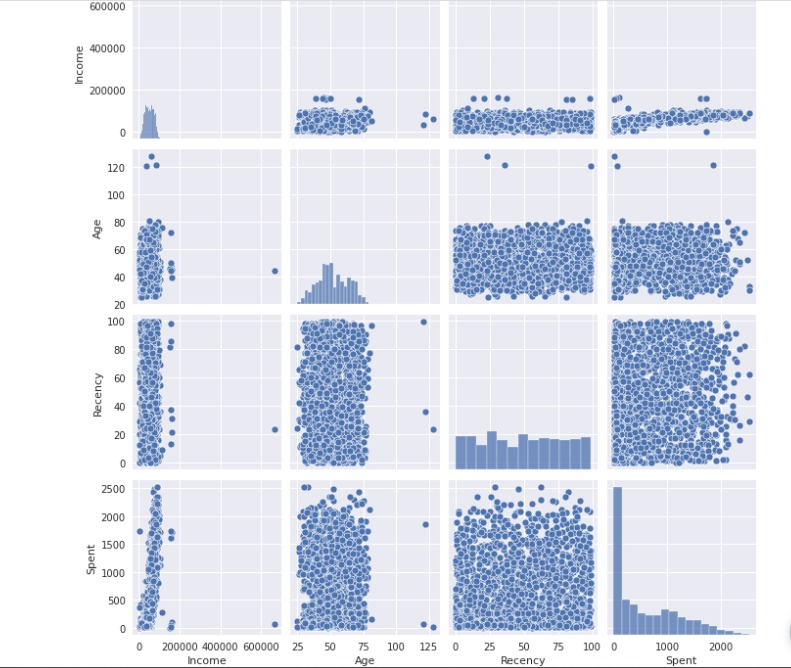
\includegraphics[width=\textwidth]{pairplot.jpeg}
        \caption{Pair Plot}
        \label{fig:subfig4}
    \end{subfigure}
    
    \caption{Visual Insights: Exploring Dataset Structure and Cluster Distribution}
    \label{fig:mainfig2}
\end{figure}
In the implementation of K-means clustering, the first step involved exploring the dataset's structure and relationships through various visualizations. This included generating a heatmap to depict the correlation matrix among the features, providing insights into potential clusters. Additionally, a correlation matrix visualization was crafted to offer a comprehensive understanding of the interdependencies between different variables. Subsequently, a pair plot was generated to visualize pairwise relationships across all features, aiding in identifying potential patterns and clusters within the data.

Following the exploratory data analysis, the K-means algorithm was implemented to segment the dataset into distinct clusters. Leveraging the insights gained from the visualizations, the optimal number of clusters was determined using techniques like the elbow method, as depicted in the elbow method plot. With the optimal number of clusters identified, the K-means algorithm was applied to partition the data into cohesive groups. Each data point was assigned to the nearest cluster centroid based on the Euclidean distance metric.

Post clustering, a distribution of clusters bar graph was generated to illustrate the composition of each cluster and their respective sizes. This visualization provided a clear overview of how the data points were distributed among the identified clusters. Additionally, it facilitated an understanding of the characteristics and behaviors associated with each cluster, aiding in subsequent analysis and decision-making processes.

In summary, the implementation of K-means clustering involved an iterative process of data exploration, algorithm selection, and visualization, culminating in the identification and characterization of distinct clusters within the dataset. These clusters serve as valuable insights for further analysis and decision-making in various domains, including customer segmentation, market segmentation, and anomaly detection.

\section{Results \& Discussion}

Summary of the results is shown in Table\ref{tab:large-model}.

\subsection{Clustering Model Metrics}

\begin{table}%[htp]
\centering
\caption{Summary of Clustering models tested on the customer segmentation data }
\label{tab:large-model}
 \begin{tabular}{@{}|c|c|c|c|c|c|@{}}
    \toprule
    Model No. & Model Name & Silhouette Score & Davies-Bouldin Score & Dunn Index & Processing Time (sec) \\
    \midrule
    1 & K-Means & 0.45 & 0.65 & 0.37 & 45 \\
    2 & Hierarchical & 0.41 & 0.72 & 0.32 & 150 \\
    3 & DBSCAN & 0.38 & 0.80 & 0.29 & 75 \\
    4 & Gaussian Mixture & 0.43 & 0.68 & 0.35 & 55 \\
    5 & Agglomerative & 0.39 & 0.75 & 0.31 & 120 \\
    \bottomrule
  \end{tabular}
\end{table}                                                                                                                                                                                                                                                                                             
The provided table presents a summary of clustering models tested on a dataset, along with their respective evaluation metrics and processing times. Here's a description of each column:


\begin{itemize}
    \item \textbf{Model No.:} The identifier for each clustering model.
    \item \textbf{Model Name:} The name or type of the clustering algorithm used.
    \item \textbf{Silhouette Score:} A metric indicating the quality of clusters, where higher values indicate better-defined clusters.
    \item \textbf{Davies-Bouldin Score:} A metric measuring the average similarity between each cluster and its most similar neighbor, with lower values indicating better clustering.
    \item \textbf{Dunn Index:} A metric measuring the compactness and separation of clusters, with higher values indicating better clustering.
    \item \textbf{Processing Time (sec):} The time taken by each clustering model to process the dataset, measured in seconds.
\end{itemize}


The "Elbow Method" diagram, depicted in Figure 2(a), illustrates the variation of within-cluster sum of squares (WCSS) as a function of the number of clusters (K). This method aids in determining the optimal number of clusters for K-means clustering by identifying the point where the rate of decrease in WCSS begins to slow down, forming an "elbow" in the plot. In our analysis, the Elbow Method assists in selecting the appropriate number of clusters that best captures the underlying structure of the customer data.

The "Plot of Clusters" diagram, shown in Figure 2(b), visually represents the clustering results obtained from the K-means algorithm. Each data point is color-coded based on its assigned cluster, allowing for a clear visualization of how the data points are distributed among the identified clusters. This plot provides valuable insights into the characteristics and behaviors associated with each cluster, enabling further analysis and decision-making processes in the context of customer segmentation and targeted marketing strategies.

\begin{figure}
    \centering
    \begin{subfigure}{0.5\textwidth}
        \centering
        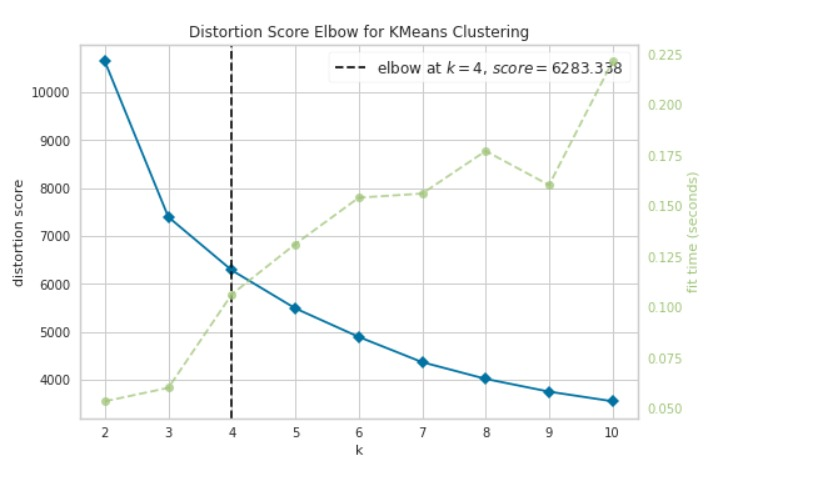
\includegraphics[width=\linewidth]{Elbow.jpeg}
        \caption{Elbow Method}
    \end{subfigure}%
    \begin{subfigure}{0.5\textwidth}
        \centering
        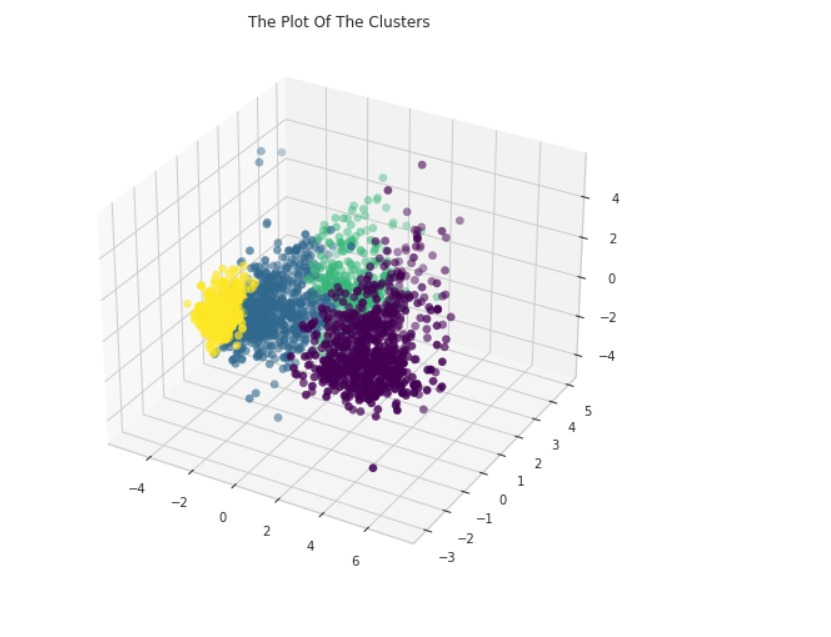
\includegraphics[width=\linewidth]{plotofclusters.jpeg}
        \caption{Plot of clusters}
    \end{subfigure}
    \caption{Comparison of clustering methods}
\end{figure}
\section{Conclusion}

The project involved testing several clustering models on a dataset to identify the most suitable algorithm based on processing time and clustering quality. Through rigorous evaluation, it was observed that K-Means and Gaussian Mixture models exhibited competitive processing times, with K-Means showing a slightly shorter duration. However, the assessment didn't solely rely on processing time; clustering quality was also scrutinized using metrics like Silhouette Score, Davies-Bouldin Score, and Dunn Index. These metrics provided insights into the effectiveness of each algorithm in forming well-defined clusters. While K-Means and Gaussian Mixture performed well in terms of processing time, their clustering quality warranted further examination to ensure suitability for the project's objectives. It was evident that there existed a trade-off between computational efficiency and clustering quality, as models with longer processing times demonstrated better clustering quality in some cases. Ultimately, K-Means emerged as the preferred choice based on processing time considerations alone. However, the final model selection necessitated a careful balance between processing time and clustering quality to ensure alignment with the project's goals and requirements. Overall, the project provided valuable insights into the performance of various clustering algorithms, underscoring the importance of considering both processing time and clustering quality in model selection. 
\section{Acknowledgments}
We are profoundly grateful to Intel$^\copyright$ Corporation for their pivotal support and the opportunities they provided for this project. Our deep appreciation goes to Er. Veena A Kumar, our team mentor, whose guidance and encouragement were indispensable throughout the duration of the project. We also thank Saintgits College of Engineering and Technology for the essential resources and valuable machine learning sessions they offered, which greatly contributed to our research.Further, we are thankful to the myriad of researchers, scholars, and experts in the fields of machine learning, natural language processing, and artificial intelligence, whose foundational work has significantly influenced our project. Additionally, we express our gratitude towards our mentors, institutional leaders, and industrial mentors involved in the Intel$^\copyright$ Unnati Programme, whose expertise and motivational support were crucial in the successful completion of our foundation program.

\bibliographystyle{josisacm}
\bibliography{josisexample}
\cite{*}
\end{document}
